\documentclass[11pt]{article}
\usepackage[margin=1in]{geometry}
\usepackage{amsmath,amssymb}
\usepackage{booktabs}
\usepackage{array}
\usepackage{longtable}
\usepackage{graphicx}
\usepackage{hyperref}
\usepackage{xcolor}
\usepackage{enumitem}
\usepackage{tikz-cd}
\usepackage{tikz}
\usetikzlibrary{arrows.meta,positioning,shapes.geometric,fit}
\usepackage{multicol}

\hypersetup{colorlinks=true,linkcolor=blue,citecolor=blue,urlcolor=blue}
\setlength{\parindent}{0pt}
\setlength{\parskip}{0.75\baselineskip}
\renewcommand{\arraystretch}{1.15}

\title{Beyond Reward Maximization: A Pressure-Driven Cognitive Architecture for Continual Cross-Domain Generalization and Stability}
\author{Likhith Sai Seemala\\RAVANA Research Initiative\\Independent Researcher\\Andhra Pradesh, India\\Email: likhith@oxiverse.com}
\date{May 25, 2026}

\begin{document}
\maketitle

\begin{center}
\textit{Author Note. This work presents a prototype cognitive architecture and internally reported benchmark results intended for exploratory cognitive-science discussion and future replication.}
\end{center}

\begin{abstract}
Continual learning systems must acquire new structure without erasing prior knowledge, transfer relational schemas across domains, and regulate behavior under uncertainty. This paper presents RAVANA (Recursive Adaptive Variable Architecture for Neurocognitive Autonomy), a pressure-driven cognitive architecture that combines a Recursive Learning Model (RLM), a typed ConceptGraph, predictive-coding style local settling, sleep-time consolidation, episodic replay, and homeostatic cognitive variables. Unlike standard reward-maximizing or end-to-end backpropagation systems, RAVANA treats error, dissonance, novelty, identity stability, and memory pressure as interacting control signals. We describe the architecture in detail and report internal benchmark results from within-domain association learning, cross-domain analogy probes, lifelong streaming retention, and synthetic fairness stress tests. In these experiments, architectural fixes raised within-domain top-1 accuracy from 0\% to 100\%; cross-domain probes reached 14.3\% top-1 and 71.4\% top-10; and a combined replay, elastic-weight-consolidation, and Bayesian edge-posterior mechanism reduced measured catastrophic forgetting from 12.0\% to 0.0\% in a 15,000-experience stream. These results should be interpreted as prototype evidence rather than final cognitive validity: the benchmarks are synthetic, the architecture is small, and independent replication is required. Nevertheless, the system offers a concrete computational hypothesis for cognitive science: robust generalization may emerge not only from reward maximization, but from regulated tensions among prediction error, structural analogy, memory consolidation, and self-stabilizing identity constraints.
\end{abstract}

\textbf{Keywords:} cognitive architecture; continual learning; predictive coding; complementary learning systems; catastrophic forgetting; analogy; sleep consolidation; self-organization

\section{Introduction}
Human cognition is not well described as a sequence of isolated supervised updates. People learn from sparse experience, reuse relational schemas across domains, preserve much of what they previously knew, sleep and rehearse, regulate uncertainty, and sometimes resist immediately rewarding actions when those actions conflict with longer-term goals or identity. These capacities motivate a long tradition in cognitive science that treats cognition as an adaptive, self-organizing, memory-dependent process rather than a purely reward-maximizing calculation \cite{hebb1949,grossberg1980,mcclelland1995,friston2010,kumaran2016}.

Modern machine learning has achieved extraordinary performance with large-scale differentiable models, especially transformers trained by backpropagation. Yet several problems remain central for cognitive science and artificial intelligence: catastrophic interference during sequential learning \cite{mccloskey1989,french1999}, weak causal or analogical transfer outside the training distribution, limited interpretability of internal structure, and difficulty integrating affective, motivational, and memory-like regulatory variables into a unified architecture. Continual-learning methods such as elastic weight consolidation, synaptic intelligence, gradient episodic memory, progressive networks, and rehearsal buffers address parts of this problem, but they often remain external additions to a task-optimized learning system \cite{kirkpatrick2017,zenke2017,lopezpaz2017,rusu2016,rebuffi2017}.

This manuscript studies RAVANA, a prototype cognitive architecture developed around a different organizing principle: cognition is governed by pressure. Prediction error, free energy, novelty, dissonance, memory salience, identity stability, confidence, and fairness tension are represented as internal variables that regulate learning and action. The model therefore does not ask only, ``Which action maximizes reward?'' It also asks whether a new update is coherent with prior structure, whether an apparent fact contradicts existing memory, whether a concept is overloaded, whether replay is needed, whether an edge is reliable, and whether a policy shift destabilizes identity.

The paper is written for a cognitive science audience. Its goal is not to claim human-level cognition or superiority over large language models. Instead, it provides a detailed architectural account, reports internal synthetic benchmarks, identifies current limitations, and frames RAVANA as a testable computational hypothesis about how local learning, graph-structured concepts, replay, predictive coding, and homeostatic governance can be integrated.

\subsection{Contributions}
The manuscript makes five contributions.
\begin{enumerate}[leftmargin=*]
    \item It specifies a pressure-driven architecture combining an RLM, typed ConceptGraph, recurrent sequence processing, predictive-coding settle loops, ConceptBinding, episodic memory, and sleep consolidation.
    \item It formalizes a governance layer in which dissonance, identity strength, uncertainty, novelty, and fairness pressure modulate learning and policy acceptance.
    \item It reports internal benchmark results on within-domain learning, cross-domain analogy, lifelong streaming retention, and bias-mitigation stress tests.
    \item It contrasts RAVANA with backpropagation-centered systems, transformer attention, state-space models, complementary learning systems, and predictive-coding accounts.
    \item It identifies failure modes and engineering gaps, including sample efficiency, speed, scaling, local-context limitations, and the need for independent validation.
\end{enumerate}

\section{Theoretical Background}
\subsection{Catastrophic Forgetting and Complementary Learning}
Sequential learning creates a stability--plasticity dilemma. A system must remain plastic enough to encode new experiences but stable enough to preserve old knowledge. Connectionist models can overwrite prior mappings when trained on new tasks, a phenomenon known as catastrophic forgetting or catastrophic interference \cite{mccloskey1989,french1999}. Complementary Learning Systems theory addresses this problem by distinguishing fast episodic learning, associated with hippocampal mechanisms, from slower integrative learning, associated with neocortical consolidation \cite{mcclelland1995,kumaran2016}. Sleep replay and offline consolidation are natural computational candidates for integrating these systems \cite{wilson1994,ji2007,diekelmann2010}.

RAVANA adopts this division architecturally. Online learning creates and updates concept edges, relation vectors, and episodic traces. Sleep-time mechanisms replay salient memories, downscale unstable edges, update confidence estimates, and consolidate repeated structure into more durable representations. The model is therefore not a single monolithic learner but an interaction between online plasticity and offline stabilization.

\subsection{Predictive Coding and Local Learning}
Predictive-coding theories propose that cortical processing minimizes local prediction errors between hierarchical levels \cite{friston2010}. These theories are attractive for cognitive architecture because they replace global error signals with locally available discrepancies. RAVANA uses this idea in its settle loop: each hidden layer compares its current state with a prediction from the layer below, updates the state locally, and gates Hebbian plasticity by local error magnitude.

This design is not equivalent to biologically faithful cortical predictive coding, nor does it provide the exact gradients of backpropagation. It is a computational compromise: local updates are less sample-efficient than backpropagation, but they permit online, streaming, interpretable, and partially modular learning.

\subsection{Analogy and Relational Transfer}
A central cognitive ability is using a relation learned in one domain to reason in another. For example, a causal schema learned from physical events may support inferences about social or emotional events if the system represents the relation independently of the surface concepts. RAVANA operationalizes this capacity through typed relation vectors, concept attention over active nodes, and relation-predictor modules that separate entity identity from relational role.

\section{Architecture}
\subsection{System Overview}
RAVANA contains three interacting layers. The first is the machine-learning substrate: embeddings, recurrent processing, hidden layers, local learning rules, concept lookup, and relation prediction. The second is the cognitive core: ConceptGraph, memory systems, contradiction detection, global workspace, self-concept tracking, and sleep consolidation. The third is a unified interface that exposes experience processing, inference, persistence, diagnostics, and consolidation.

For an input sequence $x_{1:T}$, the model performs four broad operations. First, tokens are embedded and mapped probabilistically onto concepts. Second, a recurrent cell integrates sequential context. Third, a predictive-coding settle loop updates hidden states and local prediction errors. Fourth, graph and memory systems update concept activations, typed edges, episodic traces, and homeostatic scalar variables.

\begin{figure}[htbp]
\centering
\resizebox{\textwidth}{!}{%
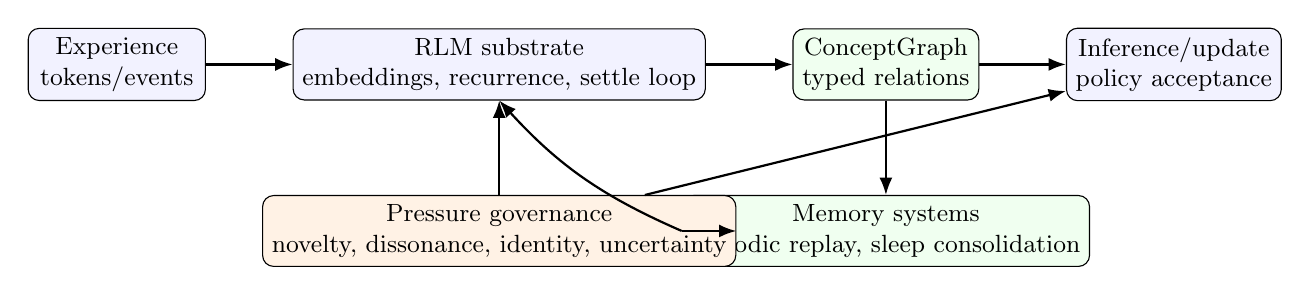
\begin{tikzpicture}[
    node distance=1.2cm and 1.1cm,
    block/.style={draw, rounded corners, align=center, minimum width=2.25cm, minimum height=0.85cm, fill=blue!5, font=\small},
    core/.style={draw, rounded corners, align=center, minimum width=2.35cm, minimum height=0.9cm, fill=green!6, font=\small},
    gov/.style={draw, rounded corners, align=center, minimum width=2.7cm, minimum height=0.9cm, fill=orange!10, font=\small},
    arrow/.style={-{Latex[length=2.2mm]}, thick}
]
\node[block] (input) {Experience\\tokens/events};
\node[block, right=of input] (substrate) {RLM substrate\\embeddings, recurrence, settle loop};
\node[core, right=of substrate] (graph) {ConceptGraph\\typed relations};
\node[core, below=of graph] (memory) {Memory systems\\episodic replay, sleep consolidation};
\node[gov, below=of substrate] (governance) {Pressure governance\\novelty, dissonance, identity, uncertainty};
\node[block, right=of graph] (action) {Inference/update\\policy acceptance};

\draw[arrow] (input) -- (substrate);
\draw[arrow] (substrate) -- (graph);
\draw[arrow] (graph) -- (action);
\draw[arrow] (graph) -- (memory);
\draw[arrow] (memory) -- (governance);
\draw[arrow] (governance) -- (substrate);
\draw[arrow] (governance) -- (action);
\draw[arrow] (memory.west) to[bend left=12] (substrate.south);
\end{tikzpicture}
}%
\caption{High-level RAVANA data flow. Online experience updates recurrent states and graph relations; memory replay and sleep consolidation stabilize repeated structure; pressure-governance variables modulate learning and policy acceptance.}
\label{fig:ravana-architecture}
\end{figure}

\subsection{ConceptGraph}
The ConceptGraph is a heterogeneous directed graph $G=(V,E)$. Nodes represent concepts, abstract clusters, episodic keys, or latent relation anchors. Edges carry typed relations such as associative, causal, inhibitory, analogical, temporal, or hierarchical. Each edge $e_{ij}$ stores at least a weight $w_{ij}$, confidence $c_{ij}$, relation type $\tau_{ij}$, age, access history, and optional Bayesian posterior parameters.

Spreading activation is precision-weighted and degree-normalized:
\begin{equation}
 a_j^{(t+1)} = \sigma\left( \sum_{i \in \mathrm{Pa}(j)} a_i^{(t)} w_{ij} c_{ij} \frac{s_{ij}}{\sqrt{\deg_{in}(j)+1}} \right),
\end{equation}
where $a_i$ is activation, $s_{ij}$ is a sign or inhibitory modifier determined by edge type, and the denominator implements fan-effect normalization. Inhibitory edges suppress incompatible alternatives, helping the graph avoid uncontrolled coactivation.

\subsection{Recurrent Processing and Gating}
Earlier RLM versions used a vanilla recurrent cell, which was too weak for temporal binding and was initially undertrained. The current architecture uses gated recurrent dynamics similar in spirit to a GRU:
\begin{align}
 z_t &= \sigma(W_z [x_t,h_{t-1}] + b_z),\\
 r_t &= \sigma(W_r [x_t,h_{t-1}] + b_r),\\
 \tilde{h}_t &= \tanh(W_h [x_t,r_t \odot h_{t-1}] + b_h),\\
 h_t &= (1-z_t)\odot h_{t-1} + z_t\odot \tilde{h}_t.
\end{align}
The update gate controls replacement of prior state, while the reset gate controls how much previous context shapes the candidate state. This is important for relational language because causal, temporal, and analogical roles often depend on earlier tokens.

\subsection{Predictive-Coding Settle Loop}
Let $h_l$ denote the hidden state at layer $l$, and let $W_l h_{l-1}$ denote the prediction generated from the previous layer. At each settling step, the layer computes a normalized local error:
\begin{equation}
 e_l = \frac{h_l - W_l h_{l-1}}{\epsilon + \lVert W_l h_{l-1}\rVert_2}.
\end{equation}
The hidden state is then adjusted:
\begin{equation}
 h_l^{(k+1)} = h_l^{(k)} - \eta_{settle}e_l^{(k)} + \xi^{(k)} + \alpha_{novelty}(h_l^{(k)}-\bar{h}_l),
\end{equation}
where $\xi$ is small Gaussian noise and $\bar{h}_l$ is a running historical state. Noise and novelty terms prevent collapse into static attractors. Layer normalization or residual normalization stabilizes activation scale.

After settling, local error gates Hebbian updates:
\begin{equation}
 \Delta W_l = \eta_{base}\left(1 + \lambda_e\lVert e_l\rVert_2 c_l\right)e_l h_{l-1}^{\top}.
\end{equation}
This rule is not a global gradient. It uses information locally available to the layer: the presynaptic activation, the postsynaptic error, and confidence or precision.

\subsection{ConceptBinding and Semantic Namespaces}
The mapping between tokens and concepts is probabilistic. A token may bind to multiple concepts, and a concept may be expressed by multiple tokens. For a token $x$, the binding map defines $p(v_k|x)$. Ambiguity is measured by entropy:
\begin{equation}
 H_{bind}(x)=-\sum_k p(v_k|x)\log p(v_k|x).
\end{equation}
High entropy indicates semantic overload. The architecture can then split concepts, create namespace-specific bindings, or delay commitment until additional context reduces uncertainty.

\subsection{Memory System and Sleep Consolidation}
RAVANA includes an episodic memory buffer, a persistent memory engine, and a bridge from memory to weights. Each experience stores content, timestamp, salience, emotional or value tags, prediction error, and concept associations. Memory strength decays over time, approximately following an Ebbinghaus-like curve:
\begin{equation}
 S_i(t)=S_i(0)\exp(-\lambda_i t),
\end{equation}
where $\lambda_i$ is smaller for salient, repeated, or high-confidence memories.

Sleep cycles perform interleaved replay. Slow-wave-like stages emphasize consolidation and synaptic homeostasis, whereas REM-like stages emphasize recombination, analogy, and contradiction testing. During replay, the model samples salient and uncertain traces, reactivates their concepts, updates edge confidence, and applies homeostatic downscaling to prevent dense graph explosion. This procedure is inspired by sleep replay and synaptic homeostasis accounts \cite{tononi2006,walker2006,diekelmann2010,wilson1994,ji2007}.

\section{Homeostatic Governance}
\subsection{Cognitive Currencies}
The architecture tracks scalar variables called cognitive currencies. These variables are not output labels; they are internal regulators. The most important are cognitive dissonance $D$, identity strength $I$, uncertainty $U$, novelty $N$, affective valence $V$, arousal $A$, dominance or control $C$, and free energy $F$.

Dissonance is an exponentially smoothed estimate of conflict between current evidence, prior beliefs, selected actions, and identity constraints:
\begin{equation}
 D_t=(1-\alpha_D)D_{t-1}+\alpha_D\left[\sum_i \left|\phi(b_i)-\phi(a_t)\right|\,\mathrm{conf}_i\,\mathrm{sal}_i+\lambda_{struct}\right].
\end{equation}
Identity strength combines stability, resistance to harmful perturbation, and conceptual coherence:
\begin{equation}
 I = 0.40\,\mathrm{stability}+0.35\,\mathrm{resistance}+0.25\,\mathrm{coherence}.
\end{equation}
These variables modulate learning rates, replay priority, action rejection thresholds, and attention allocation.

\subsection{GRACE Governor}
The governance layer, called GRACE in the implementation notes, acts as a closed-loop controller. It evaluates whether candidate updates should be accepted, attenuated, delayed, or rejected. A simplified decision score is:
\begin{equation}
 A_{update}=R + \beta_N N - \beta_D D + \beta_I I - \beta_U U - \beta_C C_{violation},
\end{equation}
where $R$ is task reward or local success, $N$ is novelty, $D$ is dissonance, $I$ is identity stability, $U$ is uncertainty, and $C_{violation}$ is a constraint-violation term. This equation illustrates the architectural principle: reward is only one pressure among several.

\subsection{Global Workspace}
A global workspace bottleneck broadcasts a small set of high-salience concepts to the rest of the system. Candidate contents compete by activation, novelty, dissonance, memory salience, and task relevance. The broadcast mechanism supports coordination among graph updates, memory retrieval, recurrent inference, and governance.

\section{Experimental Methods}
All results in this paper are internal prototype results derived from the project reports supplied with the manuscript. They should be treated as engineering evidence and hypotheses for future replication, not as independently verified cognitive-science findings.

\subsection{Model Configuration}
The reported experiments used a compact configuration: embedding dimension 32, concept dimension 32, hidden size 32, three hidden layers, five settle steps, base learning rate 0.001, free-energy threshold 8.0, sleep interval 100, and random seed 42. A word-level tokenizer was used for most concept experiments because it reduced overhead relative to BPE in small-vocabulary relational tasks.

\subsection{Within-Domain Association Learning}
The within-domain task tested whether the system could learn target associations after earlier failures. Early versions achieved 0\% top-1 accuracy because relation vectors collapsed, concepts proliferated without sufficient gating, and sleep downscaling erased useful structure. Three fixes were introduced: relation-vector type seeds and anchoring, concept-creation gating, and adaptive per-edge homeostatic downscaling.

\subsection{Cross-Domain Analogy Probes}
The cross-domain task trained the model on a science domain and evaluated transfer to an emotion domain. The purpose was to test whether relations such as ``causes'', ``produces'', or ``enables'' could be separated from surface vocabulary. An example successful probe was applying a causal schema learned from ``friction causes heat'' to infer the target in ``kindness causes trust.''

\subsection{Lifelong Streaming Benchmark}
The lifelong benchmark used a stream of 15,000 experiences across five entity epochs, with noise and contradiction rates inherited from the project configuration. The full anti-forgetting condition combined sleep-time replay, elastic-weight-consolidation penalties, and Bayesian edge posterior tracking. The baseline used pure Hebbian graph updates without the full triad.

\subsection{Fairness and Governance Stress Test}
The fairness experiment used a synthetic student-interaction dataset with $N=10{,}000$ and an initial demographic parity gap of 19.58\%. The test measured whether governance dynamics could reduce disparity without reducing success for the advantaged group.

\section{Results}
\subsection{Within-Domain Learning}
After the architectural fixes, within-domain top-1 accuracy rose from 0\% to 100\% in the reported association benchmark. The result indicates that the original failure was not simply an inherent limitation of local learning; it was caused by identifiable architectural defects in relation separation, concept growth, and sleep downscaling.

\begin{table}[h]
\centering
\caption{Within-domain learning before and after architectural fixes.}
\begin{tabular}{lcc}
\toprule
Condition & Top-1 accuracy & Primary failure or mechanism \\
\midrule
Initial RLM & 0\% & Relation collapse; concept ballooning; sleep erasure \\
Fixed RLM & 100\% & Anchored relation vectors; gated concepts; adaptive downscaling \\
\bottomrule
\end{tabular}
\end{table}

\subsection{Cross-Domain Transfer}
The RLM outperformed the backpropagation MLP baseline on the reported structural analogy probes. The strongest result was top-10 transfer: 71.4\% for the RLM versus 14.3\% for the MLP baseline in the cross-domain probe set. Top-1 remained low at 14.3\%, indicating that relational structure was often present but not ranked first.

\begin{table}[h]
\centering
\caption{Cross-domain transfer probe performance.}
\begin{tabular}{lcc}
\toprule
Metric & RLM & MLP baseline \\
\midrule
Cross-domain probe top-1 & 14.3\% & 0.0\% \\
Cross-domain probe top-10 & 71.4\% & 14.3\% \\
Fair evaluation top-1 & 14.4\% & 0.0\% \\
Fair evaluation top-10 & 48.4\% & 10.3\% \\
Fair evaluation discrimination & 0.44 & 0.08 \\
Forward transfer to Domain B & 57.1\% & 14.3\% \\
Zero-shot transfer & 57.1\% & 14.3\% \\
\bottomrule
\end{tabular}
\end{table}

\subsection{Catastrophic Forgetting}
The full anti-forgetting triad improved final retention and eliminated measured catastrophic forgetting in the 15,000-experience benchmark. Final overall retention rose from 40.8\% to 47.6\%, measured forgetting fell from 12.0\% to 0.0\%, per-step processing time decreased from 272 ms to 42 ms, and edge count fell by 64\%, suggesting a more efficient graph.

\begin{table}[h]
\centering
\caption{Lifelong streaming benchmark.}
\begin{tabular}{lccc}
\toprule
Metric & Pure Hebbian & Replay + EWC + Bayesian & Delta \\
\midrule
Final overall retention & 40.8\% & 47.6\% & +6.8 pp \\
Catastrophic forgetting & 12.0\% & 0.0\% & -12.0 pp \\
Per-step process time & 272 ms & 42 ms & 6.5$\times$ faster \\
Concepts / nodes & 384 & 384 & stable \\
Edges & 58,795 & 21,117 & 64\% fewer \\
\bottomrule
\end{tabular}
\end{table}

Retention gains were largest in epochs that suffered most under the baseline. Epoch 1 rose from 38.0\% to 52.0\%, and epoch 3 rose from 32.0\% to 52.0\%.

\begin{table}[h]
\centering
\caption{Retention by entity epoch.}
\begin{tabular}{lccc}
\toprule
Epoch & Pure Hebbian & Full triad & Delta \\
\midrule
0, early & 44.0\% & 46.0\% & +2.0 pp \\
1, new wave & 38.0\% & 52.0\% & +14.0 pp \\
2 & 44.0\% & 44.0\% & 0.0 pp \\
3, new wave & 32.0\% & 52.0\% & +20.0 pp \\
4, late & 42.0\% & 44.0\% & +2.0 pp \\
\bottomrule
\end{tabular}
\end{table}

\subsection{Fairness Stress Test}
In the synthetic student-interaction dataset, RAVANA reduced the demographic parity gap from 19.58\% to 7.81\%, a 60.1\% reduction. Both groups improved in absolute success rate: Group A rose from 79.66\% to 86.86\%, and Group B rose from 60.08\% to 79.05\%.

\begin{table}[h]
\centering
\caption{Synthetic fairness benchmark.}
\begin{tabular}{lccc}
\toprule
Metric & Raw baseline & RAVANA v2 & Change \\
\midrule
Demographic parity gap & 19.58\% & 7.81\% & 60.1\% reduction \\
Group A success & 79.66\% & 86.86\% & +7.20 pp \\
Group B success & 60.08\% & 79.05\% & +18.97 pp \\
Max group disparity & 19.58\% & 7.81\% & reduced \\
\bottomrule
\end{tabular}
\end{table}

Ablations suggest that the dissonance engine, reward rejection, and identity penalty all contributed to stability. Removing the dissonance engine produced the largest reported collapse in fairness stability.

\begin{table}[h]
\centering
\caption{Governance ablation.}
\begin{tabular}{lcc}
\toprule
Configuration & Demographic parity gap & Stability collapse \\
\midrule
Full RAVANA v2 & 7.8\% & baseline \\
No identity penalty & 11.2\% & +3.4 pp \\
No reward rejection & 14.1\% & +6.3 pp \\
No dissonance engine & 14.4\% & +6.6 pp \\
\bottomrule
\end{tabular}
\end{table}

\section{Discussion}
\subsection{What the Results Suggest}
The results support four cautious claims. First, local learning can fail catastrophically for fixable architectural reasons. The move from 0\% to 100\% within-domain accuracy was achieved not by abandoning local learning but by correcting relation collapse, uncontrolled concept creation, and sleep-time erasure. Second, relation-specific structure can support limited cross-domain transfer. The RLM's top-10 advantage over the MLP baseline suggests that typed relations and graph structure can make analogical candidates available even when ranking remains imperfect. Third, replay and consolidation are central rather than optional. The anti-forgetting triad improved both retention and graph efficiency. Fourth, governance variables can alter policy dynamics in ways that resemble internal regulation rather than external reward maximization alone.

\subsection{Relation to Cognitive Science}
RAVANA connects several cognitive-science traditions. Its graph dynamics and inhibition echo adaptive resonance and self-organizing cognitive codes \cite{grossberg1980}. Its local error minimization echoes predictive coding and free-energy accounts \cite{friston2010}. Its fast memory plus slow consolidation reflects Complementary Learning Systems theory \cite{mcclelland1995,kumaran2016}. Its sleep replay mechanisms are inspired by evidence for hippocampal and cortical memory reactivation \cite{wilson1994,ji2007,diekelmann2010}. Its global workspace module follows the idea that conscious access is a limited-capacity broadcast process \cite{baars1997}. Its governance layer extends these ideas by treating identity, dissonance, and uncertainty as computational regulators.

\subsection{Comparison with Transformers and State-Space Models}
Transformers provide global token-token attention and are highly optimized for parallel training. RAVANA is weaker in raw speed, sample efficiency, and broad language competence. However, it has explicit graph structure, online updating, typed relations, replay, and interpretable memory traces. Concept attention in RAVANA can be viewed as a sparse, graph-constrained analogue of transformer attention over active concepts rather than all tokens.

State-space models such as Mamba show that recurrent sequence models can be competitive when equipped with selective gating and efficient scan operations \cite{gu2023}. RAVANA shares the emphasis on stateful sequence processing, but it adds graph memory, local predictive settling, and cognitive governance. A natural future direction is to replace inefficient recurrent components with modern selective state-space layers while preserving graph and memory mechanisms.

\subsection{Limitations}
The limitations are substantial. The experiments are synthetic and internally reported. The architecture is small and not yet evaluated on large naturalistic cognitive benchmarks. The top-1 cross-domain transfer result remains low. Local Hebbian and predictive-coding updates are less sample-efficient than backpropagation. Graph operations can become expensive at scale, especially if pairwise curvature or similarity computations are not sampled. Earlier code audits found bugs such as undertrained recurrent cells, unused normalization, lack of gating, and inefficient generation paths; the project reports state that these were fixed, but independent verification remains necessary. Finally, the fairness benchmark is not a substitute for real-world ethical validation.

\section{Future Work}
Future work should prioritize independent replication, public benchmark definitions, and ablation-controlled evaluation. The most important technical directions are: (1) replacing brute-force graph operations with sampled or indexed approximations; (2) improving ranking so relational candidates move from top-10 to top-1; (3) integrating concept attention with modern state-space or transformer components; (4) testing on naturalistic analogy, causal reasoning, and continual-learning datasets; (5) separating cognitive plausibility claims from engineering performance claims; and (6) formalizing governance variables as measurable computational constructs.

\section{Conclusion}
RAVANA is a prototype pressure-driven cognitive architecture designed to study continual learning, analogy, memory consolidation, and self-regulation. Its central hypothesis is that cognition can be modeled as regulated interaction among prediction error, graph structure, replay, uncertainty, novelty, dissonance, and identity stability. Internal experiments show promising improvements in within-domain learning, cross-domain transfer, catastrophic-forgetting control, and synthetic fairness dynamics, but the evidence remains preliminary. For cognitive science, the value of the architecture is its explicit and testable integration of mechanisms that are often studied separately: local predictive error, structured concepts, sleep replay, global workspace broadcasting, and homeostatic governance.

\section*{Ethics, Data, and Reproducibility Statement}
The reported benchmarks are synthetic and should not be used to justify deployment in high-stakes settings. The fairness experiment is a stress test of internal regulation, not evidence of real-world fairness. A submission-ready empirical version of this paper should include code, random seeds, benchmark generation scripts, preregistered metrics, and independent baselines. Any use of generative AI assistance in drafting should be disclosed according to the target journal's author guidelines.

\begin{thebibliography}{99}
\bibitem{baars1997} Baars, B. J. (1997). \textit{In the Theater of Consciousness: The Workspace of the Mind}. Oxford University Press.
\bibitem{bengio2014} Bengio, Y. (2014). How auto-encoders could provide standardized targets for deep networks. \textit{arXiv:1407.7906}.
\bibitem{chaudhry2019} Chaudhry, A., Ranzato, M., Rohrbach, M., \& Elhoseiny, M. (2019). Efficient lifelong learning with A-GEM. \textit{International Conference on Learning Representations}.
\bibitem{diekelmann2010} Diekelmann, S., \& Born, J. (2010). The memory function of sleep. \textit{Nature Reviews Neuroscience, 11}(2), 114--126.
\bibitem{friston2010} Friston, K. (2010). The free-energy principle: A unified brain theory? \textit{Nature Reviews Neuroscience, 11}(2), 127--138.
\bibitem{french1999} French, R. M. (1999). Catastrophic forgetting in connectionist networks. \textit{Trends in Cognitive Sciences, 3}(4), 128--135.
\bibitem{grossberg1980} Grossberg, S. (1980). How does a brain build a cognitive code? \textit{Psychological Review, 87}(1), 1--51.
\bibitem{gu2023} Gu, A., \& Dao, T. (2023). Mamba: Linear-time sequence modeling with selective state spaces. \textit{arXiv:2312.00752}.
\bibitem{hebb1949} Hebb, D. O. (1949). \textit{The Organization of Behavior}. Wiley.
\bibitem{ji2007} Ji, D., \& Wilson, M. A. (2007). Coordinated memory replay in the visual cortex and hippocampus during sleep. \textit{Nature Neuroscience, 10}(1), 100--107.
\bibitem{kirkpatrick2017} Kirkpatrick, J., Pascanu, R., Rabinowitz, N., Veness, J., Desjardins, G., Rusu, A. A., et al. (2017). Overcoming catastrophic forgetting in neural networks. \textit{Proceedings of the National Academy of Sciences, 114}(13), 3521--3526.
\bibitem{kumaran2016} Kumaran, D., Hassabis, D., \& McClelland, J. L. (2016). What learning systems do intelligent agents need? Complementary learning systems theory updated. \textit{Trends in Cognitive Sciences, 20}(7), 512--534.
\bibitem{lopezpaz2017} Lopez-Paz, D., \& Ranzato, M. (2017). Gradient episodic memory for continual learning. \textit{Advances in Neural Information Processing Systems}.
\bibitem{mallya2018} Mallya, A., \& Lazebnik, S. (2018). PackNet: Adding multiple tasks to a single network by iterative pruning. \textit{IEEE Conference on Computer Vision and Pattern Recognition}.
\bibitem{mcclelland1995} McClelland, J. L., McNaughton, B. L., \& O'Reilly, R. C. (1995). Why there are complementary learning systems in the hippocampus and neocortex. \textit{Psychological Review, 102}(3), 419--457.
\bibitem{mccloskey1989} McCloskey, M., \& Cohen, N. J. (1989). Catastrophic interference in connectionist networks: The sequential learning problem. \textit{Psychology of Learning and Motivation, 24}, 109--165.
\bibitem{rebuffi2017} Rebuffi, S.-A., Kolesnikov, A., Sperl, G., \& Lampert, C. H. (2017). iCaRL: Incremental classifier and representation learning. \textit{IEEE Conference on Computer Vision and Pattern Recognition}.
\bibitem{rusu2016} Rusu, A. A., Rabinowitz, N. C., Desjardins, G., Soyer, H., Kirkpatrick, J., Kavukcuoglu, K., et al. (2016). Progressive neural networks. \textit{arXiv:1606.04671}.
\bibitem{scellier2017} Scellier, B., \& Bengio, Y. (2017). Equilibrium propagation: Bridging the gap between biophysical brains and backpropagation. \textit{Frontiers in Computational Neuroscience, 11}, 24.
\bibitem{tononi2006} Tononi, G., \& Cirelli, C. (2006). Sleep function and synaptic homeostasis. \textit{Sleep Medicine Reviews, 10}(1), 49--62.
\bibitem{walker2006} Walker, M. P., \& Stickgold, R. (2006). Sleep, memory, and plasticity. \textit{Annual Review of Psychology, 57}, 139--166.
\bibitem{wilson1994} Wilson, M. A., \& McNaughton, B. L. (1994). Reactivation of hippocampal ensemble memories during sleep. \textit{Science, 265}(5172), 676--679.
\bibitem{zenke2017} Zenke, F., Poole, B., \& Ganguli, S. (2017). Continual learning through synaptic intelligence. \textit{International Conference on Machine Learning}.
\end{thebibliography}

\end{document}
